\documentclass{article}
\usepackage[utf8]{inputenc}
\usepackage{amsmath}
\usepackage{graphicx}
\usepackage{hyperref}
\usepackage[english]{babel}\usepackage{subcaption}
\usepackage{sidecap}
\usepackage{lipsum}
\usepackage{multicol}
\usepackage{sectsty}
\usepackage{caption}
\usepackage{placeins}
\usepackage{subcaption}
\usepackage[dvipsnames]{xcolor}

\definecolor{myred}{RGB}{143, 42, 12}
\definecolor{myblue}{RGB}{58, 83, 197}
\definecolor{myorange}{RGB}{219, 146, 0}



% \sectionfont{\centering}
\usepackage[a4paper,top=2cm,bottom=2cm,left=2cm,right=2cm]{geometry}
\title{Deep Quaternion Neural Network for 3D Sound \\ Source Localization and Detection
\\ \large{\vspace{0.4cm}Project of Neural Network Course, Prof. Uncini}}
\author{Sveva Pepe 1743997 \\  Marco Pennese 1749223 \\  Claudia Medaglia 1758095}
\date{}

\begin{document}
    \maketitle
    % \begin{abstract}
    %     We work with 3D audio sounds, in particular we analyze the sound event localization and detection (SELD). 
    %     \\ We were provided with a dataset containing the sounds that were recorded with the first-order Ambisonics microphone. 
    %     These sounds are then represented using spherical harmonics decomposition in the quaternion domain, to then be passed to 
    %     the neural network which will be towed in order to obtain the best possible results in output.
    %     \\ The neural network is quaternion convolutional, with the addition of some recurrent layers.
    %     The aim of the project is to detect the temporal activities of a known set of sound event classes and to further locate them 
    %     in space by using quaternion-valued data processing.
    % \end{abstract}
    \section{Introduction}
    Sound source localization is a fundamental task, expecially in revembrant and multiple sources envoirments; it includes recognizing the temporal onset and offset of sound events when active, classifying the sound events into known set of classes, and further localizing the events in space when active using their direction of arrival (DOA).\\
    In this project, we work with 3D audio sounds captured by first-order Ambisonic microphone and these sounds are then represented 
    by spherical harmonics decomposition in the quaternion domain.
    \\ The aim of the project is to detect the temporal activities of a known set of sound event classes and to further locate them in 
    the space using quaternion-valued data processing, in particular we focus on the sound event localization and detection (SELD). 
    \\ In order to do this, we use a given Quaternion Convolutional Neural Network with the addition of some recurrent layers (QCRNN) 
    for the joint 3D sound event localization and detection task.
    % Talk about SELD, which is made up of DOA and SED. Say what I am in a general way, don't go into too much detail, don't go too 
    % far [my advice]. (they are well written in the last paper sent by our friend cominiello).
    % To say that with quaternions the performances are better than without.
    % Then do you.
    % At the end of the introduction, say what the next sections are made up of. 
    \section{Quaternion domain}
    3D audio files are sampled using the Ambisonics technique, where sampling is based on the decomposition of sound in a linear 
    combination of orthogonal bases of spherical harmonics.
    \\ In this project the first-order Ambisonics (FOA) was considered, which is composed of 4 microphone capsules. The first is
    a pressure microphone, the other three are orthogonal eight-shaped microphones related to the pressure gradient, or the acoustic
    speed.
    \\ The pressure microphone is an omnidirectional microphone that has unity gain in all directions. It is indicated by the letter W 
    and corresponds to the spherical harmonic function of order 0.
    Instead the other three microphones are denoted respectively with X, Y, Z and correspond to the harmonic functions of order 1.
    \\ Our goal is to use spherical harmonics in the quaternion domain, so let's consider four ambisonic signals, namely $x_W[n]$, 
    $x_X[n]$, $x_Y[n]$ e $x_Z[n]$, as a single quaternion signal:
    \begin{equation*}
        x[n]=x_W[n]+x_X[n]\hat{i}+x_Y[n]\hat{j}+x_Z[n]\hat{k}
    \end{equation*}
    where x[n] is quaternion-valued ambisonic signal and the four components define the B-Ambisonics format, in fact, we have:
    \begin{equation*}
        \begin{cases}
            x_W[n] = \frac{s[n]}{\sqrt{3}} \\
            x_X[n] = s[n] \cos(\theta) cos(\varphi) \\
            x_Y[n] = s[n] \sin(\theta) cos(\varphi) \\
            x_Z[n] = s[n] \sin(\varphi)
        \end{cases}
    \end{equation*}
    The factor $\frac{1}{\sqrt{3}}$ to the omnidirectional microphone allows to attenuate the average energy of that channel by 
    3 dB about on the full sphere, thus making it equal to the average energy of all the other channels.
    \\ We note that $x_W[n]$ is the real component of the quaternion signal, while the $x_X[n]$, $x_Y[n]$ and $x_Z[n]$ are 
    considered the imaginary components.
    \\ Now we have to derive the quaternion-value input features that will be passed to the network, to do this we need the
    acoustic intensity.
    \\ \\ The vector of acoustic intensity, also called sound field, is produced by average of the sound pressure, $p[n]$, and
    the particle velocity, $v[n]$, over time:
    \begin{equation*}
        I[n]=p[n] \cdot v[n]
    \end{equation*}
    In addition, the sound field provides the magnitude and direction of the flow of sound energy.
    \\ Since we are using the representation of quaternions with the B-format Ambisonic we are going to rewrite the sound 
    pressure and speed.
    \\ Sound pressure is defined by the signal captured by the omnidirectional signal, $p[n] = x_W[n]$.
    While the particle velocity is defined by the three orthogonal figure-of-eight microphone signals, $v[n]= \frac{-1}{p_0c\sqrt{3}}$ $\cdot$
    $\begin{bmatrix}
            x_X[n] \\
            x_Y[n] \\
            x_Z[n]
        \end{bmatrix}
    $
    \\ where $p_0$ is the mean density of the air and $c$ is the speed of the sound.
    \\ We express the acoustic intensity in the discrete time-frequency domain in terms of pressure $p[k,n]$ and particle with complex
    velocity $v[k, n]$, where k indicates the index of the frequency bin.
    \\ So the acoustic intensity will be equal to:
    \begin{equation*}
        \begin{matrix}
            I[k,n] = p^*[k,n] \cdot v[k,n] = I_a[k,n]+jI_r[k,n]
        \end{matrix}
    \end{equation*}
    where * denotes the complex conjugation.
    \\ $I_a$ and $I_r$ are the two components that make up the acoustic intensity, respectively the active and reactive intensity.
    \\ Active intensity is the time average of the acoustic intensity:
    \begin{equation*}
        I_a [k,n]= \Re\{ p^*[k,n]\cdot v[k,n]\} 
    \end{equation*}
    which corresponds to transport of sound energy and whose mean value is non-zero.
    \\ Reactive intensity is defined as the imaginary counterpart of active intensity:
    \begin{equation*}
        I_r [k,n]= \Im \{ p^*[k,n] \cdot v[k,n]\} 
    \end{equation*}
    which corresponds to the dissipative energy transport and whose mean value is zero.
    \\ Since the intensity vectors contain the information of theacoustical energy direction of a sound wave, the acoustic intensity
    vector can be directly used for DOA estimation, used in localization.
    \\ In theory, the sound DOA can be estimated as the opposite direction of the active intensity vector. In practice, however, 
    the estimates obtained across all time-frequency bins are inconsistent in reverberant environments.
    \\ Active intensity refers directly to DOA, while reactive intensity indicates whether a given frequency-time bin is dominated
    by sound directed by a single source, opposed to overlapping sources or reverberation. 
    \\ In this way, the active and reactive intensity vectors are both extracted from the spectrogram from each audio channel and 
    are used as separate functions.
    \\ We use both the active and reactive intensity vectors across all frequency bins in the STFT domain as input features,
    in particular,  in order to represent the active and reactive intensity vectors we encapsulate the information in two quaternions. 
    \\  Since we have three components for each intensity vector, we also consider one more channel related to the magnitude of the
    omnidirectional microphone signal in order to improve the performances of the localization task.
    \\ Input features can be expressed by the two quaternions $q_a[k,n]$ and $q_r[k,n]$:
    \begin{equation*}
            \begin{matrix}
                q_a[k,n]=\Re\{x_W^*[k,n] \cdot x_W[k,n]\} \\
                \hspace{1cm} + \Re\{x_W^*[k,n] \cdot x_X[k,n]\}\hat{i} \\
                \hspace{1cm} + \Re\{x_W^*[k,n] \cdot x_Y[k,n]\}\hat{j} \\
                \hspace{1cm} + \Re\{x_W^*[k,n]\cdot x_Z[k,n]\}\hat{k} \\
            \end{matrix}
    \end{equation*}
    \begin{equation*}
        \begin{matrix}
            q_r[k,n]=\Im\{x_W^*[k,n]\cdot x_W[k,n]\} \\
            \hspace{1cm} + \Im\{x_W^*[k,n]\cdot x_X[k,n]\}\hat{i} \\
            \hspace{1cm} + \Im\{x_W^*[k,n] \cdot x_Y[k,n]\}\hat{j} \\
            \hspace{1cm} + \Im\{x_W^*[k,n]\cdot x_Z[k,n]\}\hat{k} \\
        \end{matrix}
    \end{equation*}
    We normalize each time-frequency bin by its total energy $\epsilon_T=\epsilon_P+\epsilon_K$, where $\epsilon_P=|x_W[k, n]|^2$ 
    is the potential energy density related to the sound pressure and $\epsilon_K=\frac{1}{3}(|x_X[k, n]|^2+|x_Y[k, n]|^2+|x_Z[k, n]|^2)$ 
    is the kinetic energy density related to the particle velocity.
    \\ Now can we express the normalize quaternion inputs as:
    \begin{equation*}
        \overline{q}_a [k,n] = \frac{q_a[k,n]}{\epsilon_T} 
    \end{equation*}
    \begin{equation*}
        \overline{q}_r [k,n] = \frac{q_r[k,n]}{\epsilon_T} 
    \end{equation*}
    The proposed model receives the quaternion ambisonic recording, from which it extracts the spectrogram in terms of magnitude and phase
    components using a Hamming window of lengthvM, an overlap of 50\%, and considering only the $\frac{M}{2}$ positive frequencies without the 
    zeroth bin. herefore, from the two quaternion inputs, we obtain afeature sequence of T frames, with an overall dimension of $Tx\frac{M}{2}x8$.
    % What are quaternions, and their connection with 3D audio recorded with Ambisonic.
    % Enter the mathematical formula on the composition (that of the real part + imaginary part).
    % A minimum of considerations on active and reactive intensity, in particular
    % the role of active and reactive intensity in DOA.
    % \\ Formulas of the two "input features" with quaternions.
    \section{Network Structure}
    The model receives as input the quaternions, from which it extracts the spectrogram in terms of magnitude and phase components 
    using a Hamming window.
    \\ The network is a Quaternion Convolutional Recurrent Neural Network (QCRNN).
    In particular, we have three convolutional layers based on quaternions (QCNN), two recurrent layers (QRNN) and finally two parallel 
    outputs, both are composed of two fully-connected layers, which obviously differ in their activation functions and size that 
    receive input from previous layers.
    \\ The QCNN are composed of P filter kernels with size $3x3x8$. 
    \\ The three convolutional networks (QCNN) consist of 3 stages: Convolutional, Detector and  Pooling.
    \\ The first stage consists of the convolutional process to the inputs. Since these are quaternions, the convolutional process 
    consists of Hamilton's product:
    \begin{equation*}
        \begin{matrix}
            W \otimes x =(W_wx_w - W_xx_x - W_yx_y - W_zx_z ) \\
               \hspace{1.2cm} + (W_wx_x + W_xx_w + W_yx_z - W_zx_y )\hat{i} \\
               \hspace{1.2cm} + (W_wx_y - W_xx_z + W_yx_w + W_zx_x )\hat{j} \\
               \hspace{1.2cm} + (W_wx_z + W_xx_y - W_yx_x - W_zx_w )\hat{i}
        \end{matrix}
    \end{equation*}
    where x is the vector of the quaternions taken as input and W a generic quaternion filter matrix.
    \\ Hamilton product allows quaternion neural networks to capture internal latent relations within the features of a quaternion.
    \\ After it is applied the Batch Normalization, a technique for improving the speed, performance, and stability of artificial 
    neural networks. It is used to normalize the input layer by adjusting and scaling the activations.
    Also, batch normalization allows each layer of a network to learn by itself a little bit more independently of other layers.
    \\ The second phase concerns the choice of the activation function, which in the case of the three quaternion convolutional layer 
    is the ReLU.\footnote{ReLU stands for rectified linear unit, and is a type of activation function. Mathematically, it is defined 
    as $y = \max(0, x)$ where y is the output and x is the input.}
    \\ For a generic quaternion dense layer we have:
    \begin{equation*}
        y = \alpha( W \otimes x + b)
    \end{equation*}
    where  y is the output of the layer, b is the bias offset and $\alpha$ is quaternion activation function.
    \\ Indeed,  $\alpha(q) = f(q_w) + f(q_x) + f(q_y) + f(q_z)$, q is a generic quaternion and f is rectified linear unit (ReLU) 
    activation function. As we can see, The ReLU is applied to both the real and imaginary part of the quaternion.
    \\ \\ The last stage is the one related to Pooling. Pooling decrease the computational power required to process the data through 
    dimensionality reduction. Furthermore, it is useful for extracting dominant features which are rotational and positional invariant,
    thus maintaining the process of effectively training of the model. In our network we use MaxPooling.
    MaxPooling is done by applying a max filter to non-overlapping subregions of the initial representation.
    \\ Max-pooling is applied along the frequency axis for 
    dimensionality reduction while preserving the sequence length T, we obtain in the end that the output of the 3 QCNN has 
    dimension T x 8P and fed to bidirectional QRNN layers to better catch the time progress of the input signals.  
    \\ The network also uses the Dropout technique, which consists in randomly removing network units with some probability $\beta$.
    \\ \\ QRNN are recurring neural networks based on quaternions.
    The peculiarity of recurrent neural networks is that they differ from feedforward nets because they include a feedback loop,
    whereby output from step n-1 is fed back to the net to affect the outcome of step n, and so forth for each subsequent step.
    \\ In these QRNN Q nodes of quaternion gated recurrent units (QGRU) are used in each layer and as a function of activation
    a hyperbolic tangent (tanh).
    \\ \\ The output of the recurrent layer is shared between two fully-connected layer branches each producing the SED as 
    multi-class multilabel classification and DOA as multi-output regression; together producing the SELD output.
    \begin{figure}[htb!]
        \centering
        \fbox{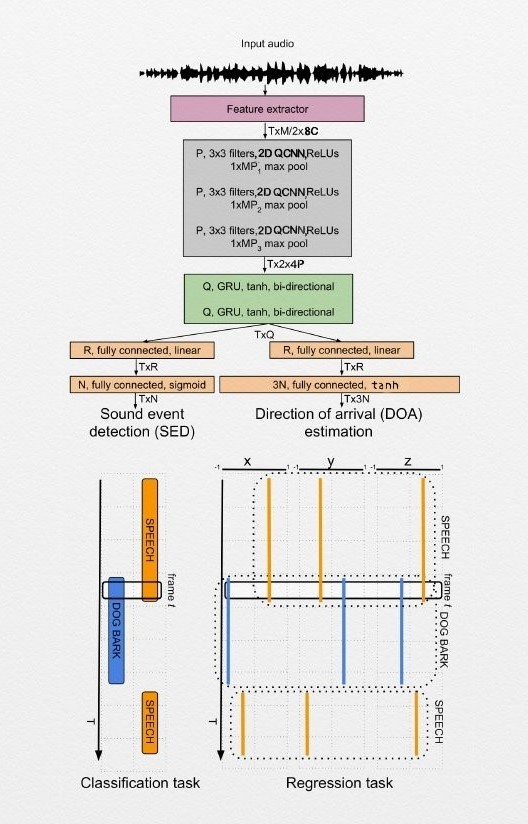
\includegraphics[width=0.5\linewidth]{images/QCRNN.jpg}}
        \caption{Quaternion Convolutional Neural Network}
        \label{fig:dqnn}
    \end{figure}
    \subsection{Weight Initialization}
    The appropriate and correct initialization of the network parameters in the quaternion domain must take into account the
    interactions between quaternion-valued components,  thus a simple random and component-wise initialization may result in an 
    unsuitable choice. 
    \\ A possible solution maybe derived by considering a normalized purely quaternion  $u^\triangleleft$ generated for each weight w 
    by following a uniform distribution in $[0,1]$. 
    \\ Each weight can be written in a polar form as:
    \begin{equation*}
        w= |w|e^{u^\triangleleft \theta} = |w| (\cos{\theta} + u^\triangleleft \sin{\theta}) 
    \end{equation*}
    from which it is possible to derive the quaternion-valued components of w:
    \begin{equation*}
        \begin{cases}
            w_W = \phi \cos{(\theta)} \\
            w_X = \phi u_X^\triangleleft\sin{(\theta)} \\
            w_Y = \phi u_Y^\triangleleft\sin{(\theta)} \\
            w_Z = \phi u_Z^\triangleleft\sin{(\theta)}
        \end{cases}
    \end{equation*}
    where $\theta$ is randomly generated in the range $[-\pi, \pi]$ and $\phi$ is a randomly generated variable related to the variance
    of the quaternion weight, defined as var(W) = $E\{|W|\} - (E\{|W|\})^2 $. where  the second term is null due to the symmetric distribution
    of the weight around 0. Since W follows a Chi distribution with four degrees of freedom, the variance can be expressed as:
    \begin{equation*}
        var(W)=E\{|W|^2\}= \int_0^\infty w^2f(w) dw = 4 \sigma^2
    \end{equation*}
    being $\sigma$ the standard deviation. The variable $\phi$ can be randomly generated in the range $[-\sigma, \sigma]$.
    % Explain the architecture, then start with the 3 QCNN, what is a convolutional network with quaternions 
    % (weights, Hamilton product etc.), which does BatchNormalization (to be specified that this is not based on quaternions), 
    % the activation functions, what is MaxPooling (just explain what it does) and conclude with the Dropout (technique that serves 
    % blah blah blah).
    % \\ Then explain the 2 QRNN recurrent layers and then what a recurrent layer is and the relationship with quaternions, very short.
    % \\ Finally say that the output of the network is doubled, making it possible to do both detection and localization. 
    % Explain the outputs with both two fully-connected layers (remember to specify the activation functions to identify that the two 
    % "outputs" are different).
    % \\I would put image of the network.
    % \\We can also specify the dimensions of the fetures after the QCNN, the QRNN and the FC.
    \section{Dataset}
    We evaluate the proposed method involving the QCRNN on a datatset, TAU Spatial Sound Events 2019 - Ambisonic, providing four-channel First-Order Ambisonic (FOA) recordings.\\
    The recordings on the dataset consist of stationary point sources from multiple sound classes each associated with a temporal onset and offset time, and DOA coordinate represented using azimuth and elevation angle.\\
    \\ The dataset consists of a development and evaluation set.  The development set consists of 400, one minute long recordings sampled at 48000 Hz, divided into four cross-validation splits of 100 recordings each. The evaluation set consists of 100 one-minute long recordings.\\
    These recordings were synthesized using spatial room impulse response (IRs) collected from five indoor locations, at 504 unique combinations of azimuth-elevation-distance. \\
    Additionally, half the number of record- ings have up to two temporally overlapping sound events, and the remaining have no overlapping.\\
    Finally, to create a realistic sound scene recording, natural ambient noise collected in the IR recording locations was added to the synthesized recordings such that the average SNR of the sound events was 30 dB.\\
    The only explicit difference between each of the development dataset splits and eval- uation dataset is the isolated sound event examples employed.\\
    The dataset consists of eleven sound event classes, each with 20 examples: knock, drawer, clearthroat, phone, keysDrop,  speech, keyboard, pageturn, cough, doorslam and laughter.\\
    The dataset contains 250 audio files, randomly divided into five splits in a way that in each split there is an equal number of examples for each class: we used the first four for training the network, while the remaining one is used for testing (20\%).
    \\ \\ We wrote a Python script in order to divide the dataset in the right way. The script automatically divides the samples and creates the directories that the the program expects to receive.
    \\ The main division is about the number of overlaps, we have samples with two and one overlap. For each one of these subsets we have two directories: one with the file audio (in wav format) and the other for the labels (in csv format). The dataset results to be divided in 4 directories. 
    \section{Metrics}
    The SELD task can use individual SED and localization (DOA) metrics.
    \\ \\ For the SED task, we use the polyphonic SED metrics that are the F-score (ideally F = 1), based on the number of true and false positives, and the error rate (ER) (ideally ER = 0), based on the total number of active sound event classes in the ground truth.\\
    A joint SED score can be considered as $S_{SED} = \dfrac{(ER+(1-F))}{2}$.
    \\ \\ On the other hand, in order to measure the performance of the localization task, a DOA estimation error DOA$_{err}$ can be used as evaluation metric, based on estimated and ground truth DOAs.\\ Moreover, a frame recall metric K (ideally K = 1) can be used based on the percentage of true positives. \\
    A joint DOA score can be defined as $S_{DOA} = \dfrac{(DOA_{err}/180 + (1 - K))}{2}$.\\
    The lower the $S_{DOA}$ score, the better the results in terms of 3D localization.
    Finally, an overall SELD score can be defined based on the previous metrics as $S_{SELD} = \dfrac{(S_{SED} + S_{DOA})}{2}$.
    \section{Experimentation}
    We did experiments using two different approaches, both by modifying the parameters and evaluating the results using a different network, and the models have been trained over 150 epochs.\\
    **After training, we computed confidence interval for each model that we created.**
    \subsection*{First Experiment}
    In the first case we trained the Quaternion based neural network with two different values for the hyperparameter of the network, in particular we changed the number of filters in the Quaternion convolutional layers, in order to discover what is the behavior of the network and its results with respect to the different parameters.\\
    To this end, we set a number of P = 32 filters in the QCNN layers of the first models, and P = 16 filters for the second ones, analyzing the results on both the datasets (with one overlap (\textbf{ov1}) and two overlaps (\textbf{ov2})).\\
    This led to a huge difference in the number of parameters of the models: in the model with P = 16 filters there are more or less 270k trainable parameters, in the model with P = 32 there are about 425k parameters.\\
    We left unchanged all the other parameters: sequence length of T = 512 frames, window length M = 512, batch size of 10, Q = 128 nodes for the recurrent networks and R = 32 nodes for the fully connected layers.
    \subsection*{Second Experiment}
    In our second experiment, we compare the proposed quaternion CRNN with the traditional approach used in this kind of problems (a SELDnet architecture based on normal convolutional layer): we found a project developed by a group of researches\footnote{ Sharath Adavanne, Archontis Politis, and Tuomas Virtanen. Github account: https://github.com/sharathadavanne/seld-dcase2019} and we trained both networks on the same dataset (TAU Spatial Sound Events 2019 - Ambisonic), distinguishing one and two overlaps with the aim of studying the results.\\
    \\
    We had to make some changes on the new network in order to adapt it to our needs. For example we couldn't extract the features in the same way of the QCRNN because the new network expects different inputs: while our network expects inputs in a Quaternion form, the traditional model expects as input some Fourier transformed values. For this reason, we had to run two different scripts for extracting the features in the two different ways. \\
    Another thing to do was to split the dataset in the same way we did before, in order to train the models on the same sets of audio files.\\
	For the rest we have left unchanged the default parameters set by the developers in their work with the Seld-net (T = 128, M = 2048, C = 4, P = 64, MP1 = MP2 = 8, MP3 = 4, Q = R = 128, N = 11).\\
	\\
	In order to provide a fair comparison, we have choosen a configuration such to have a comparable number of parameters for both the models. In particular, we used the winning configuration of our first experiment (P = 32 filters), in order to have about 425k parameters for the proposed quaternion network and about 461k parameters for the SELDnet, so the number of parameters is very similar and in this way the results are comparable. \\
    \section{Results}
	\subsection*{QCRNN with 32 filters in the Quaternion Convolutional layers}
	The results made using the neural network set with 32 filters in the convolutional layer are shown.
	\begin{figure}[hbt!]
		\centering
		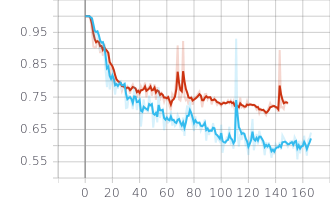
\includegraphics[height=0.34\textwidth]{images/sed_score.png} \\
		\caption{$S_{SED}$ evolution computed on the test set during the training}
	\end{figure}
	\begin{figure}[hbt!]
		\centering
		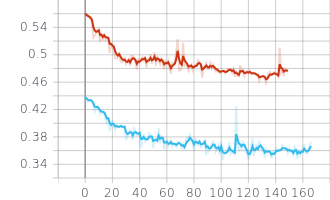
\includegraphics[height=0.34\textwidth]{images/doa_score.png} \\
		\caption{$S_{DOA}$ evolution computed on the test set during the training}
	\end{figure}
	\begin{figure}[hbt!]
		\centering
		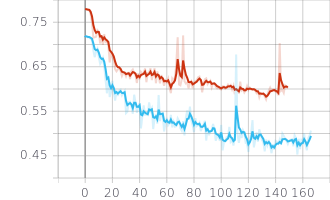
\includegraphics[height=0.34\textwidth]{images/seld_score.png}\\
		\caption{$S_{SELD}$ evolution computed on the test set during the training}
	\end{figure}
	%\FloatBarrier
	\\ \\ \\ We can see what we have achieved with the same network on both the two overlaps (ov1 and ov2). The red line refers to the 32 filter network trained on the samples with 2 overlaps (ov2), while the light blue line refers to the same network trained on samples with a single sound overlap (ov1). Indeed, what can be seen from the graphs above is that the network performs better with samples with a single overlap than that with two overlaps. This is because the second overlap makes the sound less clear and more difficult to locate and reveal.
	\\ In both cases the $S_{SED}$ score, $S_{DOA}$ score and $S_{SELD}$ score drop as the epoch increases, this means that the network continuously improves the results in order to obtain more and more better performances.
	\begin{table}[h!]
		\centering
		\begin{tabular}{c|c}
			& QCRNN \\
			\hline
			O1 \begin{tabular} {c}
				$Error\hspace{0.2cm}rate$\\
				$F1-score$ \\
				$S_{SED}$ \\
				$S_{DOA}$ \\
				$S_{SELD}$
			\end{tabular} & 
			
			\begin{tabular} {c}
				0.6122 \\
				0.4972\\
				0.5575 \\
				0.3478 \\
				0.4527 
			\end{tabular} \\
			\hline
			O2 \begin{tabular} {c}
				$Error\hspace{0.2cm}rate$\\
				$F1-score$ \\
				$S_{SED}$ \\
				$S_{DOA}$ \\
				$S_{SELD}$
			\end{tabular} & 
			\begin{tabular} {c}
				0.7529 \\
				0.3646 \\
				0.6941 \\
				0.459 \\
				0.5766
			\end{tabular}
		\end{tabular}
		\caption{The best results of the network on the TAU Dataset in terms of the SED score, DOA score and SELD score considering neural network with 32 filters in the quaternion convolutional layers. In the case of ov1 we obtained the best values in epoch 156, instead for ov2 in epoch 133.}
	\end{table}
    \subsection*{Experiments carried out: QCRNN 16, QCRNN 32 and CNN}
    \paragraph{}
	\begin{figure}[hbt!]
	\centering
	\begin{minipage}{0.5\textwidth}
	  \centering
	  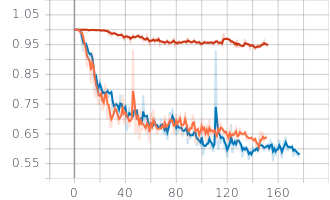
\includegraphics[width=\linewidth]{images/sed_score_ov1.png}
	  \captionof{figure}{$S_{SED}$ Score on ov1}
	\end{minipage}%
	\begin{minipage}{.5\textwidth}
	  \centering
	  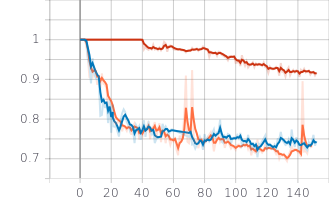
\includegraphics[width=\linewidth]{images/sed_score_ov2.png}
	  \captionof{figure}{$S_{SED}$ Score on ov2}
	\end{minipage}\\
	\vspace{1em}
	\begin{minipage}{.5\textwidth}
	  \centering
	  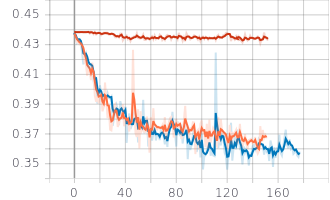
\includegraphics[width=\linewidth]{images/doa_score_ov1.png}
	  \captionof{figure}{$S_{DOA}$ Score on ov1}
	
	\end{minipage}%
	\begin{minipage}{.5\textwidth}
	  \centering
	  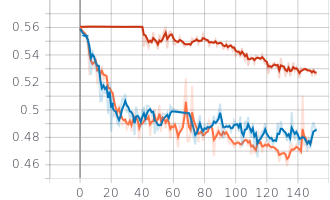
\includegraphics[width=\linewidth]{images/doa_score_ov2.png}
	  \captionof{figure}{$S_{DOA}$ Score on ov2}
	\end{minipage}\\
	\vspace{1em}
	\begin{minipage}{.5\textwidth}
	  \centering
	  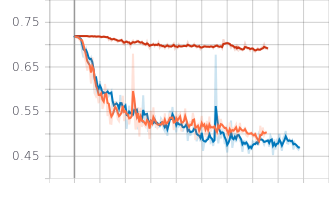
\includegraphics[width=\linewidth]{images/seld_score_ov1.png}
	  \captionof{figure}{$S_{SELD}$ Score on ov1}
	
	\end{minipage}%
	\begin{minipage}{.5\textwidth}
	  \centering
	  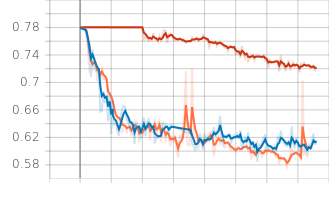
\includegraphics[width=\linewidth]{images/seld_score_ov2.png}
	  \captionof{figure}{$S_{SELD}$ Score on ov2}
	\end{minipage}\\
	\vspace{2em}

	\begin{minipage}{.45\textwidth}
	  (a) {\color{orange} \textbf{orange}}: QCRNN net with 16 filters in the quaternion convolutional layers;\\
	  (b) {\color{myblue} \textbf{blue}}: QCRNN net with 32 filters in the quaternion convolutional layers;\\
	  (c) {\color{myred} \textbf{red}}: Traditional Seld-net CRNN approach with default parameters;\\
	\end{minipage}%
	\begin{minipage}{.05\textwidth}
	  \hspace{1em}
	\end{minipage}%
	\begin{minipage}{.45\textwidth}
	  (a) {\color{myblue} \textbf{blue}}: QCRNN net with 16 filters in the quaternion convolutional layers;\\
	  (b) {\color{orange} \textbf{orange}}: QCRNN net with 32 filters in the quaternion convolutional layers;\\
	  (c) {\color{myred} \textbf{red}}: Traditional Seld-net CRNN approach with default parameters;\\
	\end{minipage}
	\end{figure} 
\FloatBarrier
	
	\begin{table}[h!]
		\centering
		\begin{tabular}{c|c|c|c}
			& QCRNN 16 & QCRNN 32 & CNN-SELDnet \\
			\hline
			O1 \begin{tabular} {c}
				$Error\hspace{0.2cm}rate$ \\
				$F1-score$ \\
				$S_{SED}$ \\
				$S_{DOA}$ \\
				$S_{SELD}$
			\end{tabular}& 
			\begin{tabular} {c}
				0.6666 \\
				0.4625 \\
				0.5976 \\
				0.3586 \\
				0.4781
			\end{tabular} & 
			\begin{tabular} {c}
				0.6122 \\
				0.4972\\
				\textbf{0.5575} \\
				\textbf{0.3478} \\
				\textbf{0.4527} 
			\end{tabular}&
			\begin{tabular} {c}
				0.9444 \\
				0.07491 \\
				0.9401 \\
				0.434 \\
				0.6843
			\end{tabular} \\
			\hline
			O2 \begin{tabular} {c}
				$Error\hspace{0.2cm}rate$ \\
				$F1-score$ \\
				$S_{SED}$ \\
				$S_{DOA}$ \\
				$S_{SELD}$
			\end{tabular}& 
			\begin{tabular} {c}
				0.7607 \\
				0.3538 \\
				0.7035 \\
				0.4655 \\
				0.5845
			\end{tabular} & 
			\begin{tabular} {c}
				0.7529 \\
				0.3646 \\
				\textbf{0.6941} \\
				\textbf{0.459} \\
				\textbf{0.5766}
			\end{tabular}&
			\begin{tabular} {c}
				0.9323 \\
				0.1126 \\
				0.9147 \\
				0.5268 \\
				0.7208
			\end{tabular} \\
		\end{tabular}
		\caption{The best results on the TAU Dataset in terms of the SED score, DOA score and SELD score considering several experiments. We considered the values referred to the best epoch for each model.}
<<<<<<< HEAD
	\end{table}	
    \section{Conclusion}
    In this work, we propose a quaternion-valued deep neural network for the localization of 3D sound events recorded by first-order Ambisonics.\\
    The proposed network involves the convolution process, as well as the rest of the processing, in the quaternion domain, thus resulting in improved performance and reduced number of parameters. The proposed method involves quaternion-valued acoustic intensity vectors as input features, which provide a more accurate DOA estimation.\\
    The method is assessed on the FOA dataset (TAU Spatial Sound Events 2019 - Ambisonic), that involves up to 2 overlapping sound events to be localized.\\
    \\
    Fixed the parameter P = 32 filters, we analyze the different results considering sounds with one or two overlaps.\\
    Of course, the models trained on the dataset with two overlaps performs worse than the models trained on the dataset with only one overlap (in splits ov2, the scores are slightly higher). In fact, having two different sound sources in the same time instant makes the problem of detecting and localizing the sources a lot more complex to solve for the network.\\
    \\
    Then we compared the QCNN with P = 32 filters and P = 16 filters.\\
    The reduction of the number of parameters results in poor performance in the proposed method, infact, we discovered that the network with P = 32 filters in the QCNN layers performs slightly better than the model with only 16 filters.\\
    \\ 
    Finally we thought it could be interesting to compare the results obtained with a SELDnet architecture based on normal convolutional layer.\\
    We set the parameters of the various models so that we find ourselves in similar situations that we can compare.\\
    Overall, as we expected, results have proved that the use of quaternion-valued acoustic intensity vector as input features leads to an improvement of 3D SELD performance in challenging environments compared to .\\
=======
\end{table}
\FloatBarrier
In the sequent plots are represented the confidence intervals for the prediction on the localization of the sound source (\textit{x} and \textit{y} coordinates) for each network tested on the different overlap.\\
\FloatBarrier
\begin{figure}[hbt!]
		\centering
		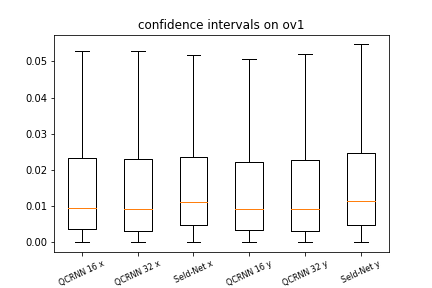
\includegraphics[width=0.6\textwidth]{images/ov1_conf.png} 
	\end{figure}
	\begin{figure}[hbt!]
		\centering
		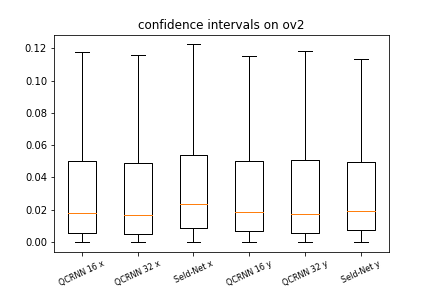
\includegraphics[width=0.6\textwidth]{images/ov2_conf.png} 
	\end{figure}

The confidence intervals of the classification error rate computed with 95\% of confidence are reported in the sequent table.\\
\FloatBarrier
\begin{table}[h!]
\centering
\begin{tabular}{c|c|c|c}
& QCRNN 16 & QCRNN 32 & CNN-SELDnet \\
\hline
O1 & $0.6610\sim 0.6647$ & $\textbf{0.6162}\sim \textbf{0.6199}$ & $0.7799\sim 0.7831$\\
\hline
O2 & $0.7541\sim 0.7574$& $\textbf{0.7512}\sim \textbf{0.7545}$& $0.7917\sim 0.7948$\\
\end{tabular}
\end{table}
\FloatBarrier
Also in this way, we can see that the best results of our experiments are reached with the QCRNN Net with 32 filters.


\section{Conclusion}
    Confronto tra i risultati ottenuti dall'esperimenti di 32. In particolare le differenze tra i due overlap (ov1 e ov2). 
    \\ Confronto tra i risultati di 16 con quelli da 32, in particolare tra i due overlap (cioè i ov1 separati da ov2). Inoltre, evidenziare che con 32 si ottengono risultati migliori. Spiegazione del perchè 32 è meglio.
    \\ Analisi complessiva delle diffenze dell'andamento della rete dei quaternioni con quella normale (CNN). In particolare, sottolineando che quella dei quaternioni risulta essere migliore e perchè.
>>>>>>> b1f1bbd77319af9e1d6d6ac631cf7b5533b2deee
\end{document}